\section{Life cycle}

	\normalsize
	{
		There are many software development models to choose from when deciding to enter into the software development process.
		The most basic of these software development models include the Waterfall model, Spiral model, V-shaped model, Iterative model
		and numerous hybrid models including the Rational Unified Process(RUP) or Model Driven Software Development(MDSD).			
		\newline
		\newline
		The choice depends largely on one key factor, the clarity of the requirements 
		\citet{CompleteDevelopmentCycle}, \citet{RequirementsVolatility}.
		From immersive reflection in the Linux management field, as a Microsoft Certified and Network Certified Professional,
		I had a good understanding of the requirements and the challenges in this project.  
		\newline
		\newline
		The formalisation of these requirements as described in Sec.\ref{sec:Scope} (Scope), indicated that many of these software development models 
		were partially applicable to the project and its goals.  As hybrid models are based around teams and parallel processes such as
		in the Rational Unified Process, these models were not applicable to this project.
		\newline
		\newline
		The choice for a static model was indicated as these offered the best match for the software development process to be carried out.	
		The waterfall model development process includes 6 stages, requirements, 
		design, implementation, testing and validation, deployment and maintenance.
		This was an appropriate candidate as these processes and their interactions are not typically 
		parallel and can be carried out by an individual.  
		\newline
		\newline
		If the requirements are not well understood or are subject to change, then the waterfall process should be avoided
		as other models such as the Rational Unified process allow for a degree of change within all stages of the software
		process being undertaken.
		\newline
		\newline
		The Waterfall model however has attracted criticisms.  One of the main criticisms is the idea of carrying out a stage of a software product's 
		life cycle perfectly and moving onto each incremental stage.  However a simple adaptation leading to an iterative waterfall process allowed me to 
		implement changes to the software product proposed. 	In Fig. \ref{fig:AdaptedWaterfallModel} the waterfall model presented shows this iterative adaptation.  
		Here we can see that the process was carried out via iterations in design, implementation, testing and deployment.
		
		\begin{multicols}{2}
		
			As the requirements were clearly established before entering into the design, development and testing stages, this mitigated the risks. 
			The risk being the cost of change, that would normally be associated with poorly scoped projects in conjunction with the waterfall model.		
			\newline
			\newline
			The cost of change through each successive stage is an exponential curve that can result in a high monetary cost; 
			if a flaw is discovered in the latter stages of the waterfall model.  A change in requirements when in the deployment
			phase could require extensive modifications to the design, implementation and resulting testing and validation stages.
			
			\vfill
			\columnbreak
		
			\begin{figurehere}
				\centering
				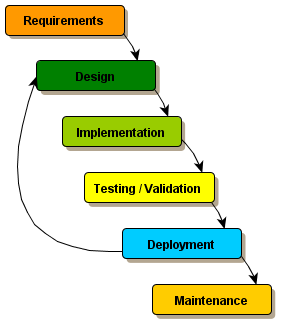
\includegraphics[scale=0.65]{pages/chapter3/figures/softwarecycle.png}
				\caption{Adapted Waterfall Model}
				\label{fig:AdaptedWaterfallModel}
			\end{figurehere}
			\vfill
			
		\end{multicols}	
		
		In the next section I will identify these requirements solidified, negating the requirement for change in the resulting development process. 
		\newline
	}
	